\section{システムの概要}
スマートモビリティレジシステムでは、エッジデバイスとなる買い物カゴにRaspberryPiと各種センサを設置する。エッジ側では商品情報(商品名、金額、賞味期限、製造日など)の特定に必要となるデータを、センサ類を用いて取得する。データの取得後サーバ側にデータを送信し、サーバ側で画像データの処理を行い、商品を特定する。システムの流れを以下の図\ref{system_summary}に示す。

\begin{figure}[htbp]
\centering
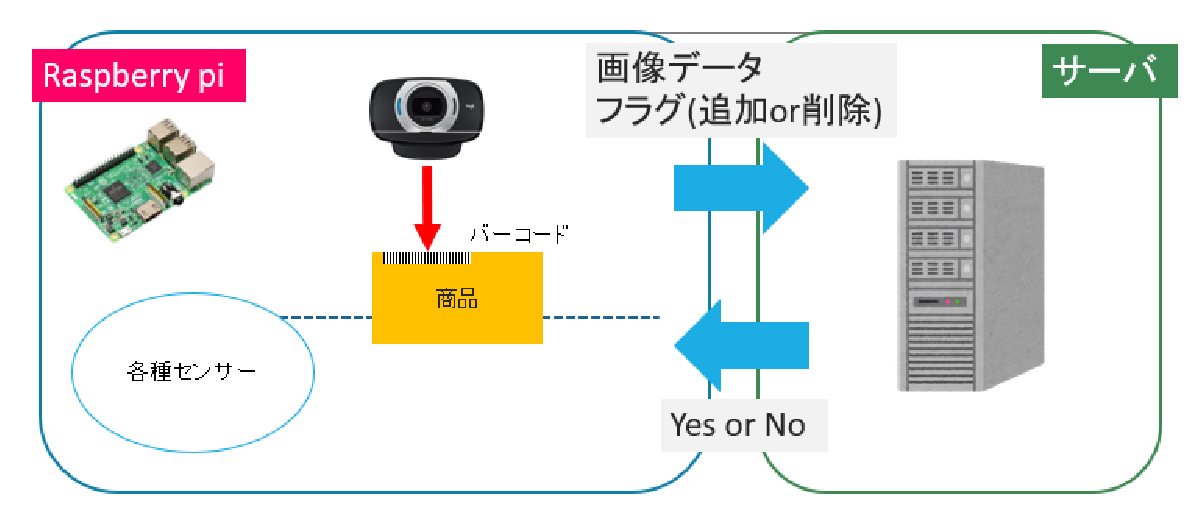
\includegraphics[width=12cm]{./pic/summary.eps}
\caption{システムの流れ}
\label{system_summary}
\end{figure}


図\ref{system_summary}の左側のRaspberryPiで商品に関するデータをサーバに送信する。フラグは、送信された画像の商品をカゴへ追加するか、削除するかどちらかを判断するために使用する。サーバは画像データとフラグを受信する。画像からバーコード番号が識別できた場合、追加・削除のフラグに従ってDBを更新する。そして、RaspberryPiに識別の結果を返信する。

